%% FullCourse_10Lecs -- Lecture 3, Topic 3.3: Forward/Backprop + Training Process
%% Source: ./archive_pre_split/Lec03_ML_for_Macro.tex (sections 4-6)
%% Pass B: layer in refinements from
%%         ../../MiniCourse_8hr/Slides/Module1_ML_Foundations/M1_T3_PyTorch_Training.tex

%% Shared preamble for the FullCourse_10Lecs topic decks.
%%
%% Each topic .tex \input's this file, then defines its own \title, \date
%% override (if any), \graphicspath, and \begin{document}.
%%
%% Reconstructed verbatim from the inlined copy preserved in
%% Lec10_Case_Studies/Lec10_T8_Case6_DeepRamsey.tex (lines 23-190), which is
%% explicitly annotated there as "from ../shared_preamble.tex, copied verbatim".
%% Base preamble matches MiniCourse_8hr/Slides/shared_preamble.tex; this version
%% additionally provides \sectiondivider, the conceptbox/cautionbox/examplebox/
%% takeawaybox tcolorboxes, and \compacttables used across the split decks.

\documentclass[10pt,english,aspectratio=169]{beamer}

\usepackage{ae,aecompl}
\usepackage[T1]{fontenc}
\usepackage{textcomp}
\usepackage[utf8]{inputenc}
\usepackage{babel}
\usepackage{datetime2}

\setcounter{secnumdepth}{3}
\setcounter{tocdepth}{3}

\usepackage{amsmath, amssymb, amsthm, graphicx}
\usepackage{booktabs, multirow}
\usepackage{tikz}
\usepackage{pgfplots}
\pgfplotsset{compat=1.16}
\usepackage[most]{tcolorbox}
\tcbuselibrary{skins, breakable, theorems}
\usepackage{listings}
\usepackage{xcolor}

\lstset{
  basicstyle=\ttfamily\small,
  keywordstyle=\color{blue!80!black}\bfseries,
  commentstyle=\color{green!50!black}\itshape,
  stringstyle=\color{orange!80!black},
  backgroundcolor=\color{gray!8},
  frame=single,
  rulecolor=\color{gray!40},
  breaklines=true,
  showstringspaces=false,
  numbers=none,
}

\lstdefinestyle{pythonstyle}{
    language=Python,
    basicstyle=\ttfamily\footnotesize,
    keywordstyle=\color{blue!80!black}\bfseries,
    commentstyle=\color{green!50!black}\itshape,
    stringstyle=\color{orange!80!black},
    frame=single,
    breaklines=true,
    showstringspaces=false,
    numbers=left,
    numbersep=5pt,
    numberstyle=\tiny\color{gray},
    backgroundcolor=\color{gray!8},
    rulecolor=\color{gray!40}
}

\ifx\hypersetup\undefined
  \AtBeginDocument{%
    \hypersetup{bookmarks=false,breaklinks=true,pdfborder={0 0 0},colorlinks=true,
      linkcolor=DarkText,urlcolor=RedTitle}%
  }
\else
  \hypersetup{bookmarks=false,breaklinks=true,pdfborder={0 0 0},colorlinks=true,
    linkcolor=DarkText,urlcolor=RedTitle}%
\fi

\makeatletter
\newcommand\makebeamertitle{%
  \begin{frame}[plain]
    \vspace*{1.0cm}
    \centering
    {\usebeamerfont{title}\usebeamercolor[fg]{title}\inserttitle\par}
    \vspace{1.0cm}
    {\usebeamerfont{author}\usebeamercolor[fg]{author}\insertauthor\par}
    \vspace{0.2cm}
    {\usebeamerfont{date}\usebeamercolor[fg]{date}\insertdate\par}
  \end{frame}}%
\AtBeginDocument{%
  \let\origtableofcontents=\tableofcontents
  \def\tableofcontents{\@ifnextchar[{\origtableofcontents}{\gobbletableofcontents}}
  \def\gobbletableofcontents#1{\origtableofcontents}%
}

\usetheme{metropolis}
\usefonttheme{professionalfonts}

\definecolor{LightGray}{RGB}{230,230,230}
\definecolor{RedTitle}{RGB}{0,0,200}
\definecolor{VeryLightGray}{RGB}{245,245,245}
\definecolor{DarkText}{RGB}{0,0,0}

\setbeamercolor{background canvas}{bg=white}
\setbeamercolor{title}{fg=RedTitle}
\setbeamercolor{author}{fg=DarkText}
\setbeamercolor{date}{fg=DarkText}
\setbeamercolor{frametitle}{bg=VeryLightGray,fg=DarkText}
\setbeamercolor{normal text}{fg=DarkText}
\setbeamerfont{title}{size=\large}

\setbeamersize{text margin left=5mm, text margin right=5mm}
\addtobeamertemplate{frametitle}{}{\vspace{-0.5em}}
\newcommand{\reducevspace}{\vspace{-0.5cm}}

% Shared section divider and box styles for split topic decks.
\newcommand{\sectiondivider}[2]{%
\begin{frame}[plain,noframenumbering]
\begin{center}
\vfill
{\Large\textbf{#1}\par}
\vspace{0.35cm}
{\normalsize #2\par}
\vfill
\end{center}
\end{frame}
}

\newtcolorbox{conceptbox}[1][]{
  colback=blue!3,
  colframe=RedTitle!55,
  boxrule=0.35mm,
  arc=1mm,
  left=2mm,
  right=2mm,
  top=1mm,
  bottom=1mm,
  #1
}
\newtcolorbox{cautionbox}[1][]{
  colback=red!3,
  colframe=red!50!black,
  boxrule=0.35mm,
  arc=1mm,
  left=2mm,
  right=2mm,
  top=1mm,
  bottom=1mm,
  #1
}
\newtcolorbox{examplebox}[1][]{
  colback=green!3,
  colframe=green!45!black,
  boxrule=0.35mm,
  arc=1mm,
  left=2mm,
  right=2mm,
  top=1mm,
  bottom=1mm,
  #1
}
\newtcolorbox{takeawaybox}[1][]{
  colback=VeryLightGray,
  colframe=RedTitle!55,
  boxrule=0.35mm,
  arc=1mm,
  left=2mm,
  right=2mm,
  top=1mm,
  bottom=1mm,
  #1
}
\newcommand{\compacttables}{\renewcommand{\arraystretch}{1.15}}

\setbeamertemplate{navigation symbols}{}
\setbeamertemplate{footline}{%
  \hfill%
  \usebeamercolor[fg]{page number in head/foot}%
  \usebeamerfont{page number in head/foot}%
  \insertframenumber\,/\,\inserttotalframenumber\kern1em\vskip2pt%
}

\makeatother

\author{Zhigang Feng}
% "date with time": compile timestamp so each build is identifiable.
\date{\today\ \DTMcurrenttime}


\graphicspath{{./pic/}{../../MiniCourse_8hr/Slides/Module1_ML_Foundations/pic/}{../}}

% Suppress the redundant auto-generated metropolis section page; the
% \sectiondivider frames below are the dividers we keep.
\metroset{sectionpage=none}
\usetikzlibrary{positioning,arrows.meta,shapes,calc}
%% Lec03 shared MAP slide: "one map, four acts" recurring diagram.
%% Input this file AFTER ../shared_preamble.tex (needs RedTitle, VeryLightGray,
%% DarkText) and AFTER \usetikzlibrary{positioning,arrows.meta,shapes,calc}.
%% Call \LecThreeMap{k} inside a frame, where k in {1,2,3,4} highlights the
%% current act ("you are here") and k = 0 renders the closing reprise with all
%% four acts checked green (used by T4's closing frame).
%% Filename deliberately does NOT match the build glob Lec*_T*.tex, so the build
%% script never tries to compile it standalone.
%%
%% The four acts are the lecture's story: WHY -> BUILD -> TRAIN -> SHAPE, i.e.
%% the case for ML in economics, the network as an object (architecture + UAT),
%% the learning machinery (backprop + SGD + regularization + double descent),
%% and economics-aware architectures with the hands-on lab.

\newcommand{\LecThreeMap}[1]{%
% Precompute per-box style selectors; TikZ option lists are comma-split before
% TeX conditionals run, so \ifnum must not sit inside a [...] options list.
\ifnum#1=0
  \tikzset{lmapa/.style={lmapdone}, lmapb/.style={lmapdone},
           lmapc/.style={lmapdone}, lmapd/.style={lmapdone}}%
\else
  \tikzset{lmapa/.style={}, lmapb/.style={}, lmapc/.style={}, lmapd/.style={}}%
  \ifnum#1=1 \tikzset{lmapa/.style={lmapcur}}\fi
  \ifnum#1=2 \tikzset{lmapb/.style={lmapcur}}\fi
  \ifnum#1=3 \tikzset{lmapc/.style={lmapcur}}\fi
  \ifnum#1=4 \tikzset{lmapd/.style={lmapcur}}\fi
\fi
\begin{center}
\begin{tikzpicture}[
    act/.style={rectangle, rounded corners, draw=black!60, fill=VeryLightGray,
        minimum width=3.0cm, minimum height=0.95cm, text width=2.9cm,
        align=center, font=\small, text=DarkText},
    lmapcur/.style={draw=RedTitle, very thick, fill=orange!20},
    lmapdone/.style={draw=green!45!black, thick, fill=green!10},
    q/.style={font=\tiny\itshape, text width=3.0cm, align=center, text=black!70},
    barlab/.style={font=\tiny\bfseries, text=black!65},
    sat/.style={rectangle, rounded corners, draw=black!45, dashed, fill=white,
        text width=5.2cm, align=center, font=\tiny, text=black!70,
        minimum height=0.5cm},
    arr/.style={-{Stealth[length=2.2mm]}, thick, gray!60}
]
    % --- four act boxes ---
    \node[act, lmapa] (a1) at (0,0)
        {\textbf{3.1\ \ WHY}\\[1pt] \tiny the case for ML in econ};
    \node[act, lmapb] (a2) at (3.6,0)
        {\textbf{3.2\ \ BUILD}\\[1pt] \tiny neurons $\cdot$ activations $\cdot$ UAT};
    \node[act, lmapc] (a3) at (7.2,0)
        {\textbf{3.3\ \ TRAIN}\\[1pt] \tiny backprop $\cdot$ SGD $\cdot$ dbl.\ descent};
    \node[act, lmapd] (a4) at (10.8,0)
        {\textbf{3.4\ \ SHAPE}\\[1pt] \tiny ICNN $\cdot$ monotone $\cdot$ lab};
    \draw[arr] (a1) -- (a2);
    \draw[arr] (a2) -- (a3);
    \draw[arr] (a3) -- (a4);
    % --- the student question each act answers ---
    \node[q] at (0,-0.95)    {why should an economist\\ care about ML?};
    \node[q] at (3.6,-0.95)  {what is a neural network,\\ and why does it work?};
    \node[q] at (7.2,-0.95)  {how does it learn ---\\ and why not overfit?};
    \node[q] at (10.8,-0.95) {how do I build economics\\ in --- and run it myself?};
    % --- "you are here" marker above the current act ---
    \ifnum#1=1 \node[font=\scriptsize\bfseries, text=RedTitle] at (0,0.98)
        {you are here\ $\blacktriangledown$};\fi
    \ifnum#1=2 \node[font=\scriptsize\bfseries, text=RedTitle] at (3.6,0.98)
        {you are here\ $\blacktriangledown$};\fi
    \ifnum#1=3 \node[font=\scriptsize\bfseries, text=RedTitle] at (7.2,0.98)
        {you are here\ $\blacktriangledown$};\fi
    \ifnum#1=4 \node[font=\scriptsize\bfseries, text=RedTitle] at (10.8,0.98)
        {you are here\ $\blacktriangledown$};\fi
    \ifnum#1=0 \node[font=\scriptsize\bfseries, text=green!45!black] at (5.4,0.98)
        {all four acts complete};\fi
    % --- bottom band: the ML pipeline (the technical spine of the lecture) ---
    \fill[blue!10]   (-1.55,-1.72) rectangle (5.15,-1.40);
    \fill[green!12]  (5.65,-1.72)  rectangle (8.75,-1.40);
    \fill[orange!16] (9.25,-1.72)  rectangle (12.35,-1.40);
    \node[barlab] at (1.8,-1.56)  {REPRESENT\ (UAT $\cdot$ Barron)};
    \node[barlab] at (7.2,-1.56)  {OPTIMIZE\ (loss $\cdot$ gradient)};
    \node[barlab] at (10.8,-1.56) {GENERALIZE $+$ CONSTRAIN};
    % --- dashed satellites: where this lecture sits in the course flow ---
    \node[sat] at (1.5,-2.42)
        {\textit{upstream:} Lec01--02 --- AI as cognitive capital; deep learning as the engine of the predictive stack};
    \node[sat] at (9.3,-2.42)
        {\textit{downstream:} Lec04--06 --- these networks become Bellman/Euler solvers for dynamic macro models};
\end{tikzpicture}
\end{center}
}


\title[AI for Econ Research]{AI for Economic Research: Dynamic Models, Language, and Agents\\
Lecture 3.3: Forward Propagation, Backpropagation \& Training}

\begin{document}

\makebeamertitle

%=============================================================================
\begin{frame}{Lecture 3 in One Map}
\textbf{One lecture, four decks, one goal: make neural networks a working tool for economists --- why they matter, what they are, how they learn, and how to make them respect economics.}

\LecThreeMap{3}

\vspace{0.05cm}
\footnotesize\textit{\textbf{Act 3.3 (here)} is the engine room: the forward pass computes predictions, backpropagation organizes the chain rule, SGD/Adam descend the loss, regularization disciplines the fit --- and double descent explains why over-parameterization helps rather than hurts.}
\end{frame}

%=============================================================================
\section{Forward Propagation}

\sectiondivider{Forward Propagation}{From input to prediction, one affine-plus-activation layer at a time}

\begin{frame}{Feedforward: Computing Outputs Layer by Layer}
\begin{itemize}
\item \textbf{Forward propagation} (feedforward): compute the network output given an input by passing through layers sequentially.

\medskip
\item For a network with $L$ hidden layers:
\[
\mathbf{h}^{(0)} = \mathbf{x}, \qquad
\mathbf{h}^{(\ell)} = \sigma\!\left(W^{(\ell)}\mathbf{h}^{(\ell-1)} + \mathbf{b}^{(\ell)}\right), \quad \ell = 1,\ldots,L
\]
\[
\hat{\mathbf{y}} = W^{(L+1)}\mathbf{h}^{(L)} + \mathbf{b}^{(L+1)}
\]

\medskip
\item Each layer: (1) multiply by weight matrix, (2) add bias, (3) apply activation.

\medskip
\item \textbf{Analogy:} Forward propagation is like solving a recursive model forward in time --- given initial state $x$, compute successive transformations to arrive at the output.
\end{itemize}
\end{frame}

\begin{frame}{Forward Pass: Visual}
\begin{center}
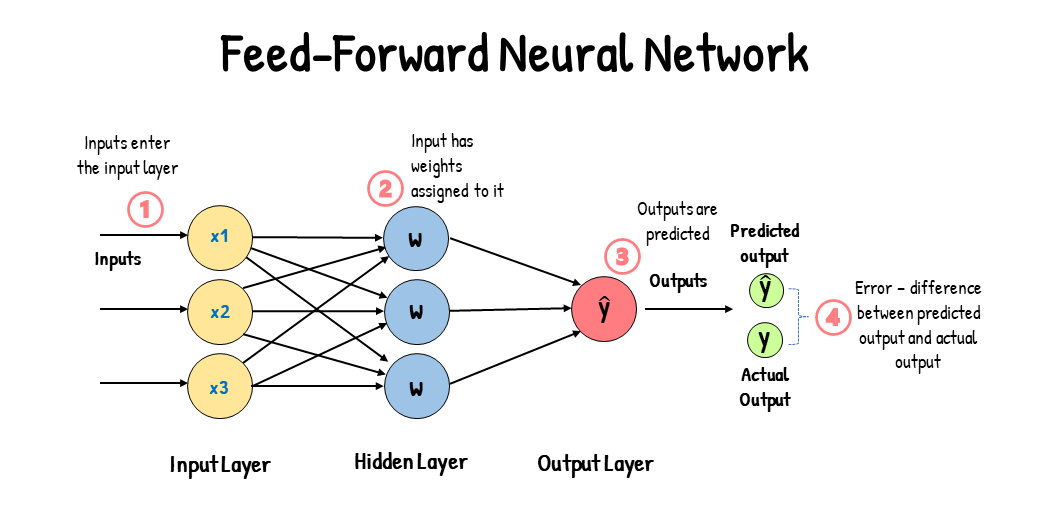
\includegraphics[width=12cm]{nn_working1}
\end{center}
\end{frame}

\begin{frame}{Toy Example: Training a Digit Classifier on One Sample}
\textbf{Recall from Lec.\ 3 T1:} we motivated ML with handwritten digit recognition.

\medskip
The toy numbers on the next slide come from the simplest version of that classifier:
\begin{itemize}
\item \emph{Input} $x$: one feature from a single digit image (in practice, the flattened 784-dim $28\times28$ pixel vector).
\item \emph{Hidden + output:} sigmoid neurons producing $\hat{y}\in[0,1]$ --- the predicted probability that the image is, say, a ``3''.
\item \emph{Target} $t$: the true label (1 if it \emph{is} a 3, 0 otherwise).
\item \emph{Loss} $L$: squared error (used here for clarity; in practice cross-entropy).
\end{itemize}

\medskip
\textbf{Why one sample?} The math is the same as training on millions: one forward pass, one loss, one backward pass, one update --- then repeat.
\end{frame}

\begin{frame}{Toy Example: Forward Pass with Numbers}
A tiny network makes every step visible: input $x=1.0$, one sigmoid hidden neuron, one sigmoid output neuron.
\vspace{-1mm}
\begin{columns}[T]
\begin{column}{0.5\textwidth}
\textbf{The network, in full:}
\[ z_1 = w_1 x + b_1,\qquad h=\sigma(z_1) \]
\[ z_2 = w_2 h + b_2,\qquad \hat{y}=\sigma(z_2) \]
\[ L=\tfrac12(\hat{y}-t)^2 \]
{\footnotesize Parameters $w_1{=}0.5,\ b_1{=}0,\ w_2{=}2.0,\ b_2{=}0$; target $t{=}0$.}
\smallskip

\textbf{With the numbers:}
\[ z_1=0.5 \;\Rightarrow\; h=\sigma(0.5)\approx0.62 \]
\[ z_2=1.24 \;\Rightarrow\; \hat{y}=\sigma(1.24)\approx0.78 \]
\[ L=\tfrac12(0.78)^2\approx0.30 \]
\end{column}
\begin{column}{0.5\textwidth}
\textbf{Reading the numbers:}
\begin{itemize}
\item Sigmoid $\sigma$ is a \emph{soft on/off switch}: $z_1{=}0.5\Rightarrow h{=}0.62$, so the hidden neuron is ``62\% on.''
\item $\hat{y}=0.78$ is the network's \emph{predicted probability} that the image is a ``3.''
\item But the truth is $t=0$ (it is \emph{not} a 3): the model is \textbf{confidently wrong} $\Rightarrow$ loss $\approx0.30$.
\item \textbf{Learning} $=$ nudge $w_1,w_2$ so $\hat{y}$ moves toward $t$. \emph{How much} each moves is what backprop computes next.
\end{itemize}
\end{column}
\end{columns}
\end{frame}

%=============================================================================
\section{Backpropagation and Gradient Descent}

\sectiondivider{Backpropagation and Gradient Descent}{The chain rule, organized: how a network computes its own gradients}

\begin{frame}{Backpropagation: Learning from Errors}
\begin{itemize}
\item \textbf{Goal:} Compute $\frac{\partial L}{\partial \theta}$ for every parameter $\theta$ in the network.

\medskip
\item \textbf{Method:} Apply the \textbf{chain rule} backwards through the network layers.

\medskip
\item \textbf{Steps:}
\begin{enumerate}
\item Forward pass: compute all activations and the loss
\item Backward pass: propagate error signal from output to input
\item Compute gradient of loss w.r.t.\ each weight and bias
\item Update parameters: $\theta \leftarrow \theta - \eta \cdot \nabla_\theta L$
\end{enumerate}
\end{itemize}

\begin{center}
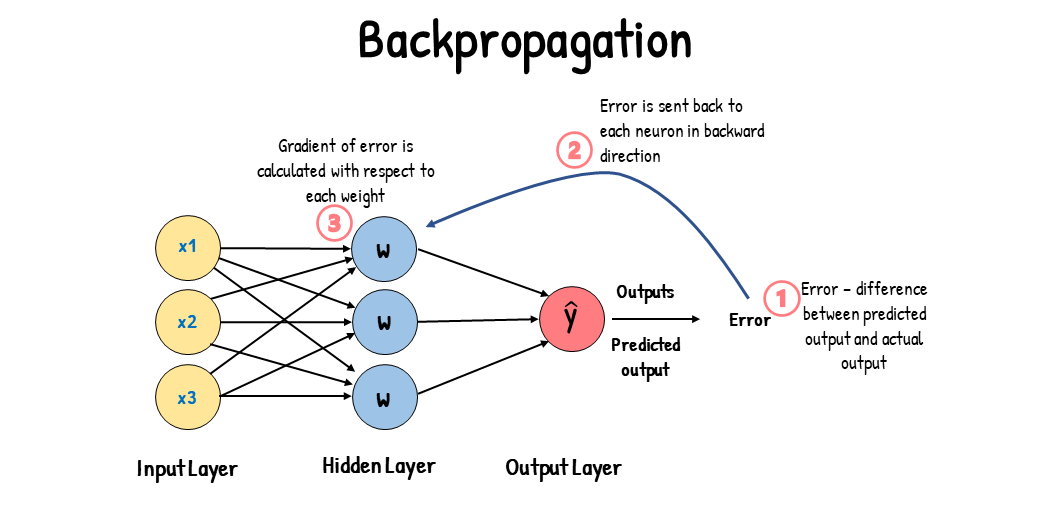
\includegraphics[width=10cm]{nn_working3}
\end{center}
\end{frame}

\begin{frame}{Toy Example: Backpropagation --- Output Layer}
\footnotesize
\textbf{The whole network in five lines} --- same example ($x=1.0,\ t=0,\ w_1=0.5,\ w_2=2.0,\ b_1=b_2=0$):
\[
z_1=w_1x+b_1,\quad h=\sigma(z_1),\quad z_2=w_2h+b_2,\quad \hat{y}=\sigma(z_2),\quad L=\tfrac12(\hat{y}-t)^2 .
\]
Forward gave $h\approx0.62,\ \hat{y}\approx0.78,\ L\approx0.30$. Backprop builds $\partial L/\partial w_2$ then $\partial L/\partial w_1$ by the \textbf{chain rule}, output layer first.
\smallskip
\begin{columns}[T]
\begin{column}{0.6\textwidth}
\textbf{Chain the links $w_2\to z_2\to\hat{y}\to L$:}
\[
\frac{\partial L}{\partial w_2}
=\underbrace{\frac{\partial L}{\partial \hat{y}}}_{\hat{y}-t}\,
\underbrace{\frac{\partial \hat{y}}{\partial z_2}}_{\hat{y}(1-\hat{y})}\,
\underbrace{\frac{\partial z_2}{\partial w_2}}_{h}
= 0.78\times0.17\times0.62\approx0.08
\]
The first two factors reusably combine into the \textbf{error signal}
\[
\delta_2\equiv\frac{\partial L}{\partial z_2}=(\hat{y}-t)\,\hat{y}(1-\hat{y})\approx0.13,
\]
so $\dfrac{\partial L}{\partial w_2}=\delta_2\,h$ and $\dfrac{\partial L}{\partial b_2}=\delta_2\approx0.13$. \emph{(We reuse $\delta_2$ for the hidden layer next.)}
\end{column}

\begin{column}{0.4\textwidth}
\centering
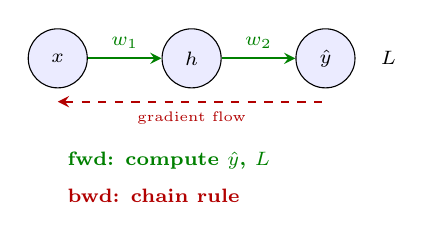
\begin{tikzpicture}[
    every node/.style={font=\scriptsize},
    layer/.style={circle, draw, minimum size=0.75cm, inner sep=0pt},
    fwd/.style={->, >=stealth, green!50!black, thick},
    bwd/.style={<-, >=stealth, red!70!black, thick, dashed},
]
\node[layer, fill=blue!8] (x) at (0,0) {$x$};
\node[layer, fill=blue!8] (h) at (1.7,0) {$h$};
\node[layer, fill=blue!8] (y) at (3.4,0) {$\hat{y}$};
\node at (4.2,0) {$L$};

\draw[fwd] (x) -- (h) node[midway, above]{$w_1$};
\draw[fwd] (h) -- (y) node[midway, above]{$w_2$};

\draw[bwd] (0, -0.55) -- node[midway, below, font=\tiny]{gradient flow} (3.4, -0.55);

\node[green!50!black, font=\scriptsize\bfseries, anchor=west] at (0, -1.3) {fwd: compute $\hat{y}$, $L$};
\node[red!70!black, font=\scriptsize\bfseries, anchor=west] at (0, -1.75) {bwd: chain rule};
\end{tikzpicture}

\smallskip
\raggedright\textbf{Read it:} $\partial L/\partial w_2>0$, so nudging $w_2$ up would \emph{raise} $L$ --- descent \emph{decreases} $w_2$ (the output overshot $t{=}0$).
\end{column}
\end{columns}
\end{frame}

\begin{frame}{Toy Example: Backpropagation --- Hidden Layer \& Update}

\textbf{Propagate the error signal back one layer} (from the output slide, $\delta_2\equiv\partial L/\partial z_2\approx0.13$):
\[
\frac{\partial L}{\partial h}
= \underbrace{\frac{\partial L}{\partial z_2}}_{\delta_2} \cdot w_2
= 0.13 \times 2.0 \approx 0.26
\]
\[
\frac{\partial h}{\partial z_1} = h(1-h)
\approx 0.62 \times 0.38 \approx 0.24
\quad\Rightarrow\quad
\delta_1\equiv\frac{\partial L}{\partial z_1}
= \frac{\partial L}{\partial h}\cdot\frac{\partial h}{\partial z_1}\approx 0.06
\]
\[
\frac{\partial L}{\partial w_1}
= \delta_1 \cdot x
= 0.06 \times 1.0 \approx 0.06
\]

\medskip
\textbf{Parameter update} (learning rate $\eta = 0.1$):
\[
w_2^{\text{new}} \approx 2.0 - 0.1 \times 0.08 = 1.992, \qquad
w_1^{\text{new}} \approx 0.5 - 0.1 \times 0.06 = 0.494
\]

\medskip
\textbf{Key point:} This is exactly what PyTorch's \texttt{.backward()} and the optimizer do --- just at massive scale with millions of parameters.
\end{frame}

\begin{frame}{Gradient Descent: The Optimization Engine}

\begin{itemize}
\item \textbf{Core update rule:}
$\theta_{n+1} \leftarrow \theta_n - \lambda_n \, g(b_n; \theta_n)$

\medskip
\item \textbf{Variants by batch size $n$:}
\begin{itemize}
\item $n=1$: \textbf{Stochastic Gradient Descent (SGD)} --- one random sample per step
\item $n=N$: \textbf{Full Gradient Descent (GD)} --- all data per step
\item $1 < n < N$: \textbf{Mini-batch GD} --- the practical sweet spot
\end{itemize}

\medskip
\item \textbf{Stochastic gradient approximation:}
\[
\frac{d\mathcal{L}(\Gamma_{\gamma})}{d\gamma} \approx \frac{1}{n}\sum_{i=1}^{n} \frac{d\mathcal{L}(\Gamma_{\gamma}; b_i)}{d\gamma}
\]

\medskip
\item \textbf{Algorithm:}
\begin{enumerate}
\item Initialize parameters randomly
\item Draw random mini-batch $b_n$; compute stochastic gradient $g(b_n; \theta_n)$
\item Choose learning rate $\lambda_n > 0$; update $\theta_{n+1} \leftarrow \theta_n - \lambda_n \, g(b_n; \theta_n)$
\item Repeat until convergence
\end{enumerate}
\end{itemize}
\end{frame}

\begin{frame}{Gradient Descent: Visual}
\begin{center}
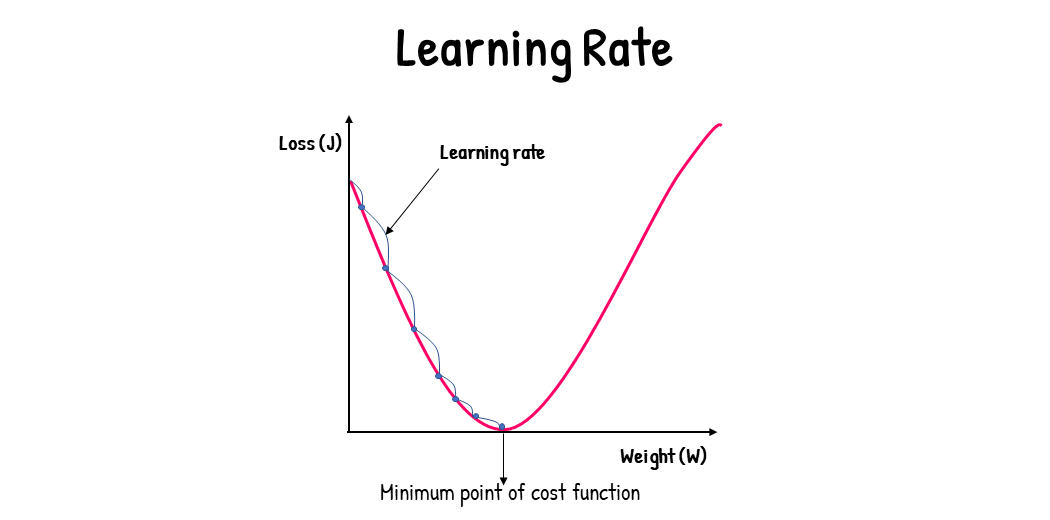
\includegraphics[width=12cm]{nn_working6}
\end{center}
\end{frame}

\begin{frame}{Adaptive Learning Rates: RProp $\to$ RMSProp $\to$ Adam}
\begin{itemize}
\item \textbf{RProp} (Riedmiller \& Braun, 1993): a \emph{full-batch} method that sizes each parameter's step from the \emph{sign} of its gradient alone --- robust, but the signs get too noisy under mini-batching.
\item \textbf{RMSProp} (Hinton, 2012): RProp adapted to mini-batches --- give each parameter its own step by dividing by a running average of \emph{squared} gradients:
\begin{align*}
g_{k} &\leftarrow \frac{1}{n}\sum_{i=1}^{n}\nabla\mathcal{L}(\Gamma_{\gamma}; b_i), \qquad
r_{k+1} \leftarrow \rho\, r_k + (1-\rho)\, g_k \odot g_k \\
\Delta\theta_{k+1} &= -\frac{\lambda}{\sqrt{\delta + r_{k+1}}} \odot g_k
\qquad\text{(big-gradient directions damped, small ones amplified).}
\end{align*}
\item \textbf{Adam} (Kingma \& Ba, 2015): momentum $+$ RMSProp --- tracks moving averages of the gradient (1st moment) and squared gradient (2nd moment); decay rates $\rho_1,\rho_2$.
\end{itemize}
\smallskip
\begin{takeawaybox}\small
\textbf{``Dominant default through $\sim$2022''} means: from its 2015 debut until roughly 2022, Adam was the optimizer nearly everyone reached for \emph{by default}, with no tuning --- the safe out-of-the-box choice --- before AdamW and others (next slide) displaced it for large models.
\end{takeawaybox}
\end{frame}

% FullCourse Pass B addition: ports MiniCourse M1_T3 modern optimizer landscape.
\begin{frame}{Beyond Adam: The Modern Optimizer Landscape (2024--2026)}
\begin{itemize}
\item \textbf{AdamW} (Loshchilov \& Hutter, 2019): decoupled weight decay; the de-facto default for transformers.
\medskip
\item \textbf{Lion} (Chen et al.\ 2023): sign-based update; lower memory than Adam, competitive on large models.
\medskip
\item \textbf{Sophia} (Liu et al.\ 2023): cheap second-order optimizer using a diagonal Hessian estimate; faster pre-training convergence.
\medskip
\item \textbf{Schedule-free optimizers} (Defazio et al.\ 2024): remove the learning-rate schedule altogether --- the optimizer self-regulates.

\medskip
\item \textbf{Course default for all labs (5A/5B, 6A/6B):} \texttt{torch.optim.AdamW(lr=1e-3, weight\_decay=1e-2)}. Vary only when explicitly noted.

\medskip
\item \textbf{Economist's take:} optimizer choice is the ML analogue of which numerical solver to use --- the right pick depends on problem geometry. For macro-scale networks ($10^3$--$10^6$ params), AdamW is the safe default.
\end{itemize}
\end{frame}

\begin{frame}{Batch vs.\ Stochastic vs.\ Mini-Batch}
\begin{center}
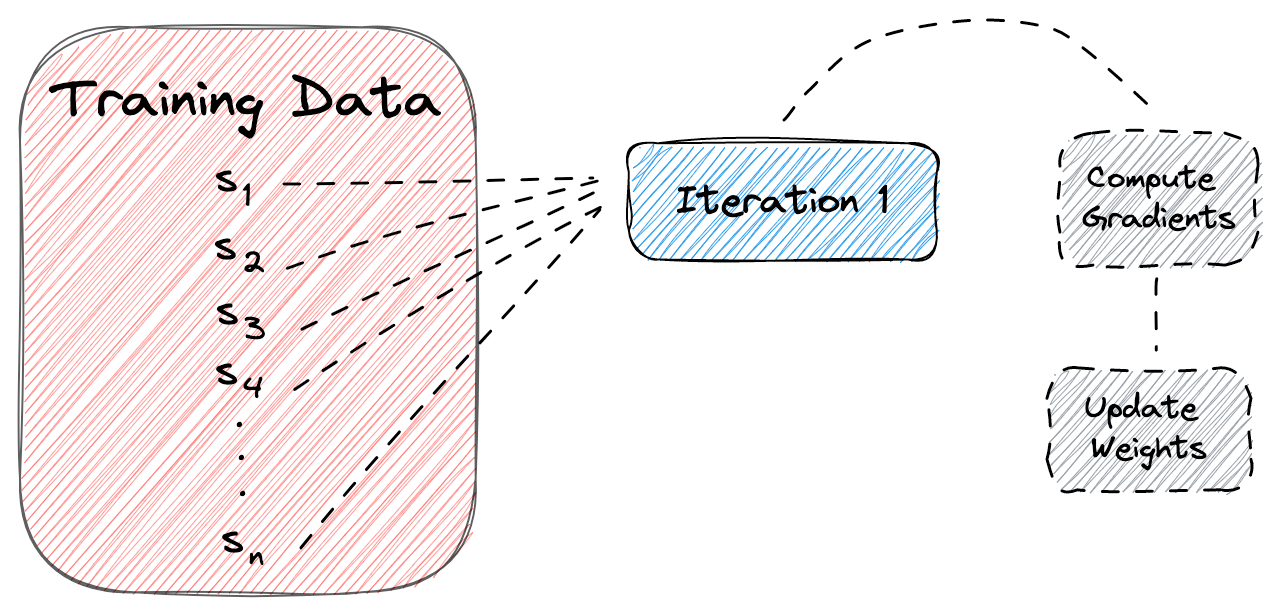
\includegraphics[width=12cm]{batch_1}
\end{center}
{\small \textbf{Batch GD:} Smooth convergence path, but each step is expensive (uses all data).}
\end{frame}

\begin{frame}{Stochastic Gradient Descent}
\begin{center}
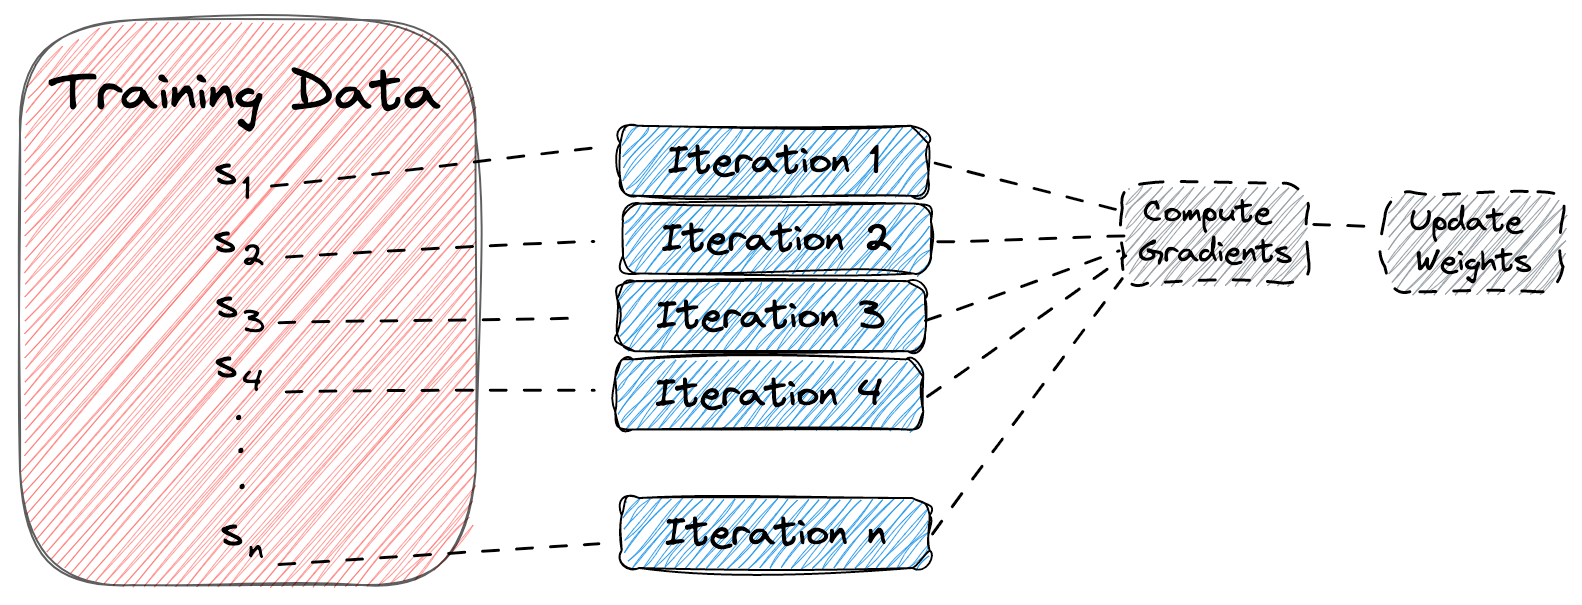
\includegraphics[width=12cm]{batch_2}
\end{center}
{\small \textbf{SGD:} Noisy path with high variance, but each step is cheap and can escape local minima.}
\end{frame}

\begin{frame}{Mini-Batch Gradient Descent}
\begin{center}
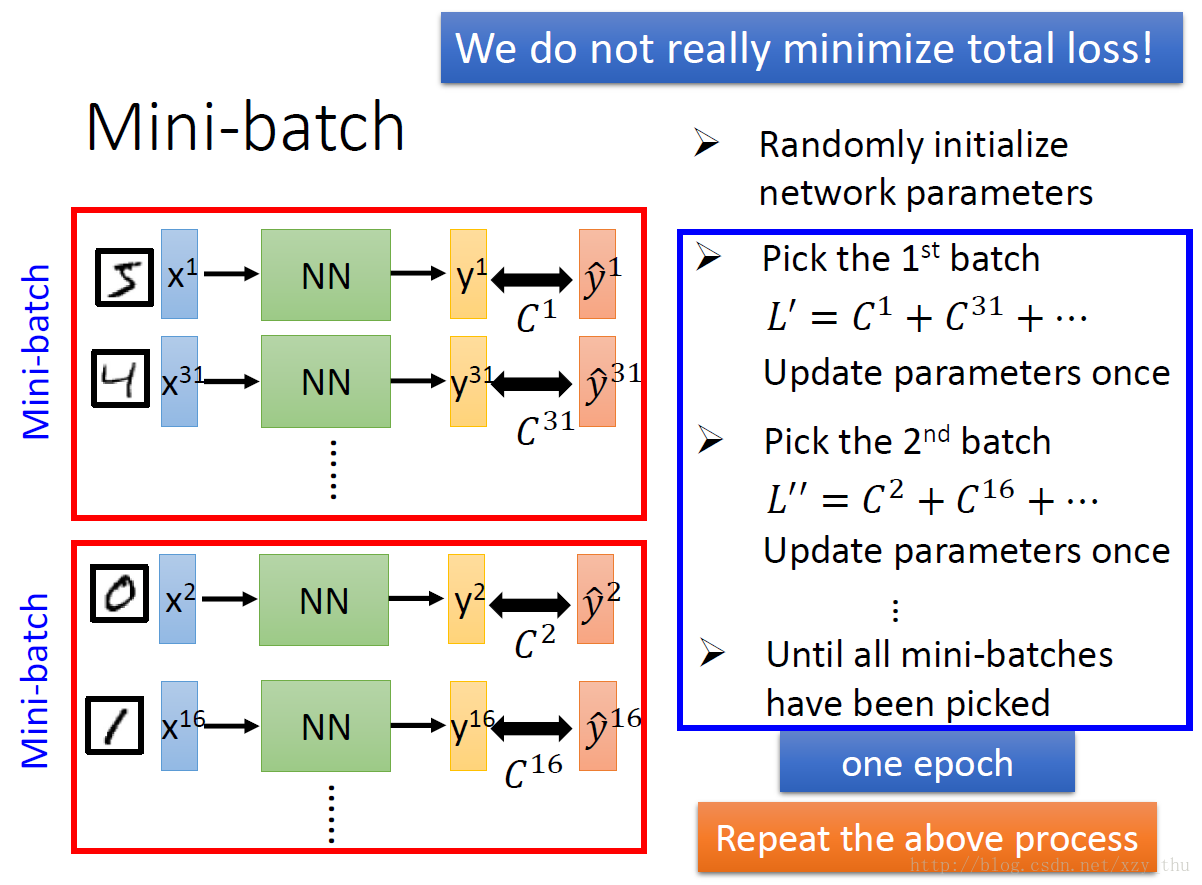
\includegraphics[width=12cm]{minibatch}
\end{center}
{\small \textbf{Mini-batch:} Balances speed (parallelizable) and stability (averaged gradients). The practical standard.}
\end{frame}

\begin{frame}{Why Mini-Batch? Four Reasons}
\begin{enumerate}
\item \textbf{Computational efficiency:} More frequent parameter updates than full GD; faster convergence in wall-clock time.

\medskip
\item \textbf{Memory constraints:} Large datasets may not fit in GPU memory. Mini-batches process manageable subsets.

\medskip
\item \textbf{Implicit regularization:} The stochasticity in gradient estimates helps escape local minima and saddle points --- acts as a form of regularization.

\medskip
\item \textbf{Parallelization:} Each mini-batch can be processed across multiple GPUs simultaneously.
\end{enumerate}

\medskip
\textbf{Economist's note:} Mini-batch SGD is the computational analogue of sampling-based estimation in econometrics --- trade exactness for speed, and the noise is actually helpful.
\end{frame}

\begin{frame}{Convergence Theory: The Guarantee}
\begin{tcolorbox}[colback=blue!3, colframe=blue!40, title=Convergence with a Diminishing Learning Rate]
\small
Under standard assumptions (Lipschitz gradient, bounded gradient-noise variance), if the learning-rate sequence satisfies
\[
\sum_{n=1}^{\infty}\lambda_n = \infty \qquad\text{and}\qquad \sum_{n=1}^{\infty}\lambda_n^2 < \infty ,
\]
then the running-average expected squared gradient vanishes:
\[
\mathbb{E}\!\left[\frac{1}{\Delta_N}\sum_{n=1}^{N}\lambda_n \|\nabla F(\theta_n)\|^2\right] \xrightarrow{N\to\infty} 0 ,
\qquad \Delta_N = \sum_{n=1}^N \lambda_n .
\]
{\footnotesize --- Bottou, Curtis \& Nocedal (2018). \textit{Optimization Methods for Large-Scale ML}.}
\end{tcolorbox}
\vspace{-1mm}
\begin{itemize}
\item \textbf{In words:} with the step size shrinking at the right rate, SGD drives its \emph{average} gradient to zero --- it settles at a stationary point. \emph{Why} each of the two conditions is needed: next slide.
\end{itemize}
\end{frame}

\begin{frame}{Convergence Theory: The Robbins--Monro Conditions, Intuitively}
The two conditions are the \textbf{Robbins--Monro conditions} (Robbins \& Monro, 1951), foundation of \emph{stochastic approximation} --- driving a noisy signal to its root. That is exactly SGD: the mini-batch gradient is a \emph{noisy estimate} of the true gradient.
\vspace{-1mm}
\begin{columns}[T]
\begin{column}{0.5\textwidth}
\begin{conceptbox}
\small\textbf{$\displaystyle\sum \lambda_n=\infty$ --- ``go the distance.''}
Steps must sum to infinity so the iterate can travel \emph{any} distance to reach the optimum, however far the start. If $\lambda_n$ decays too fast, the total path length is finite and training \textbf{stalls short}.
\end{conceptbox}
\end{column}
\begin{column}{0.5\textwidth}
\begin{conceptbox}
\small\textbf{$\displaystyle\sum \lambda_n^2<\infty$ --- ``kill the noise.''}
Squared steps must be summable so accumulated \emph{gradient noise} stays finite and dies out. This forces $\lambda_n\to0$ fast enough that late steps stop bouncing and the iterate \textbf{settles}.
\end{conceptbox}
\end{column}
\end{columns}
\vspace{-1mm}
\begin{itemize}\small
\item \textbf{Concretely:} $\lambda_n=1/n$ satisfies both ($\sum 1/n=\infty$, $\sum 1/n^2=\pi^2/6<\infty$) --- the textbook schedule. $\lambda_n=1/\sqrt{n}$ satisfies the first but \emph{fails} the second (too noisy). A \emph{constant} $\lambda$ also fails the second --- SGD then bounces forever in a ball around the optimum (early exploration, not final convergence).
\item \textbf{Econometrics link:} the same Robbins--Monro recursion underlies stochastic approximation and recursive/online estimation. \emph{ICNN-constrained training (T4; Lec.\ 4 T4) restores convergence for value/cost-function applications.}
\end{itemize}
\end{frame}

%=============================================================================
\section{Training Process: Loss Functions, Overfitting, Regularization}

\sectiondivider{Training Process: Loss, Overfitting, Regularization}{Choosing the loss and taming overfitting --- the ML analogue of disciplined econometrics}

\begin{frame}{Loss Functions I: Regression (Mean Squared Error)}
\begin{itemize}
\item \textbf{Mean Squared Error (MSE)} --- the loss for \emph{continuous} targets:
\[
\mathcal{L}_{\text{MSE}} = \frac{1}{N}\sum_{i=1}^N (\hat{y}_i - y_i)^2
\]
the average squared gap between prediction $\hat{y}_i$ and target $y_i$. Big misses are penalized quadratically.

\medskip
\item \textbf{Why this form?} Minimizing MSE is \emph{exactly} maximum likelihood under Gaussian errors --- for a linear model it \emph{is} OLS. The loss is not arbitrary: it encodes an assumption about the noise.

\medskip
\item \textbf{When to use it:} GDP growth, yields, prices, and (Lec.\ 4) Euler-equation residuals --- anything real-valued.

\medskip
\item \textbf{Economist's bridge:} MSE $\Leftrightarrow$ OLS / Gaussian MLE. Swap the noise model and you get other losses: Poisson $\to$ count data, quantile (pinball) $\to$ quantile regression.
\end{itemize}
\end{frame}

\begin{frame}{Loss Functions II: Classification (Cross-Entropy)}
\footnotesize
\textbf{Setup.} A classifier chooses among $K$ \emph{classes} --- for handwritten digits, $K=10$ (the labels $0,1,\dots,9$). The network emits a raw score $z_k$ per class; \textbf{softmax} turns the scores into probabilities that sum to one:
\[
\hat{y}_k=\text{softmax}(z)_k=\frac{e^{z_k}}{\sum_{j=0}^{K-1}e^{z_j}},\qquad \sum_{k=0}^{K-1}\hat{y}_k=1 .
\]
\textbf{The label is ``one-hot.''} The ground truth $y=(y_0,\dots,y_{K-1})$ is a vector with a single $1$ at the \emph{true} class and $0$ everywhere else --- ``one-hot'' $=$ exactly one entry hot. A true ``3'' is $y=(0,0,0,\underset{k=3}{1},0,\dots,0)$.
\smallskip
\begin{columns}[T]
\begin{column}{0.54\textwidth}
\textbf{Cross-entropy loss:}
\[
\mathcal{L}_{\text{CE}}=-\sum_{k=0}^{K-1} y_k \log \hat{y}_k \;=\; -\log \hat{y}_{k^\star}
\]
Because $y$ is one-hot, every term vanishes except the true class $k^\star$: \textbf{CE is just the negative log-probability the model assigned to the \emph{correct} answer.} Minimizing it $=$ maximizing that probability.
\end{column}
\begin{column}{0.46\textwidth}
\textbf{Why this shape is right:}
\begin{itemize}
\item true-class prob $\hat{y}_{k^\star}{=}0.99\Rightarrow L{=}-\log0.99\approx0.01$ (tiny)
\item $\hat{y}_{k^\star}{=}0.1\Rightarrow L{=}-\log0.1\approx2.3$ (large)
\item confident \emph{and} right $\to$ near $0$; confident \emph{but} wrong $\to$ blows up.
\end{itemize}
\end{column}
\end{columns}
\smallskip
\begin{takeawaybox}\footnotesize
\textbf{Economist's bridge:} this is \emph{exactly} McFadden's (1973) multinomial-logit MLE --- softmax is the logit choice probability, one-hot $y$ is the observed choice, minimizing CE is maximizing the log-likelihood. \emph{Classification $=$ discrete choice.} (Our binary toy digit was the $K{=}2$ case; softmax generalizes it to all ten digits.)
\end{takeawaybox}
\end{frame}

\begin{frame}{Training Terminology}
\begin{itemize}
\item \textbf{Epoch:} One complete pass through the entire training dataset.

\medskip
\item \textbf{Mini-batch:} A small subset of training data used for one gradient update.

\medskip
\item \textbf{Iteration:} One parameter update (= one mini-batch processed).
\begin{itemize}
\item If dataset has 10,000 samples and batch size is 100, one epoch = 100 iterations.
\end{itemize}

\medskip
\item \textbf{Automatic Differentiation:} Computational technique for exact gradient computation --- the engine behind \texttt{loss.backward()} in PyTorch.

\medskip
\item \textbf{Episode:} (Reinforcement learning context) One sequence of steps from initial state to terminal state --- analogous to one simulated life-cycle path.
\end{itemize}
\end{frame}

\begin{frame}{Overfitting and Stopping Criteria}
\begin{itemize}
\item \textbf{The fundamental tension:}
\begin{itemize}
\item Training loss: always decreasing with more epochs
\item Validation loss: decreases, then \textbf{increases} $\to$ overfitting
\end{itemize}

\medskip
\item \textbf{Stopping criteria:}
\begin{enumerate}
\item Fixed number of epochs (simple but suboptimal)
\item Monitor validation loss --- stop when it stops improving
\item \textbf{Early stopping:} halt training when validation loss increases for $k$ consecutive epochs
\end{enumerate}

\medskip
\item \textbf{Model selection:} Choose the model (epoch checkpoint) with best validation performance.

\medskip
\item \textbf{Economist's analogy:} Overfitting is the ML version of data mining --- the model memorizes noise in the training sample rather than learning the true data-generating process. Out-of-sample validation is the discipline.
\end{itemize}
\end{frame}

\begin{frame}{Local Optima vs.\ Global Optimum}
\begin{itemize}
\item \textbf{Non-convex loss landscape:}
\begin{itemize}
\item Neural network loss functions are \emph{not} convex --- many local optima and saddle points
\item Global optimum exists but is generally unreachable in practice
\end{itemize}

\medskip
\item \textbf{Mitigation strategies:}
\begin{itemize}
\item Random initialization of weights (different starting points)
\item Momentum and adaptive learning rates (escape shallow minima)
\item Mini-batch stochasticity (natural exploration of the loss surface)
\end{itemize}

\medskip
\item \textbf{Practical reality:} Finding the global optimum is neither necessary nor desirable. A \emph{good local optimum} that generalizes well is sufficient.

\smallskip
\item \textbf{Is this still the research frontier?} No --- the ``benign landscape'' result (over-parameterized nets: most local minima perform similarly; Choromanska et al., 2015) is now \emph{standard}, not frontier. The live frontier: \emph{mode connectivity} (minima joined by near-constant-loss paths --- Garipov et al.\ 2018; Frankle et al.\ 2020) and \emph{why} over-parameterization helps (\emph{double descent} --- Belkin et al.\ 2019, next section). The question is now \emph{which} minima generalize, not whether good ones exist.
\end{itemize}
\end{frame}

\begin{frame}{Regularization: Preventing Overfitting}
\begin{itemize}
\item \textbf{L1 / L2 Regularization (weight decay):}
\[
\mathcal{L}_{\text{reg}} = \mathcal{L}_{\text{data}} + \lambda \|\theta\|_p, \quad p \in \{1, 2\}
\]
\begin{itemize}
\item L1 ($p=1$): promotes sparsity (like LASSO in econometrics)
\item L2 ($p=2$): shrinks weights toward zero (like Ridge regression)
\end{itemize}

\medskip
\item \textbf{Dropout:} Randomly set a fraction of neurons to zero during each training step.
\begin{itemize}
\item Forces the network to learn redundant representations
\item Equivalent to training an ensemble of sub-networks
\end{itemize}

\medskip
\item \textbf{Batch Normalization:} Normalize activations within each layer across the mini-batch. Stabilizes and accelerates training.

\medskip
\item \textbf{Data Augmentation:} Expand the training set with transformed copies (rotation, scaling, noise injection).
\end{itemize}
\end{frame}

%=============================================================================
\section{Modern Twist: Double Descent and the Blessings of Dimensionality}

\sectiondivider{Modern Twist: Double Descent}{Why over-parameterized networks generalize --- and what that buys economic modelling}

\begin{frame}{The Modern Twist: Double Descent}
\textbf{The ``validation loss turns up $\Rightarrow$ overfitting'' story (two slides ago) is only the \emph{under-parameterized} half of the picture.}
\smallskip
\begin{center}
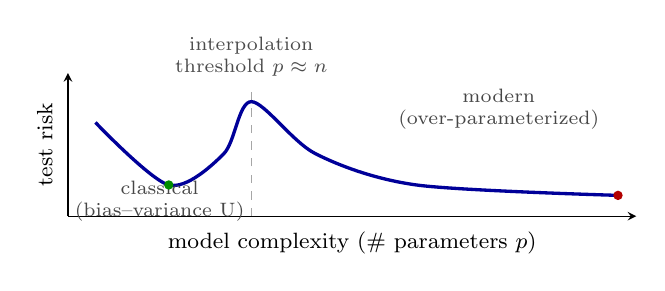
\begin{tikzpicture}
\begin{axis}[
  width=8.8cm, height=3.4cm,
  xlabel={\footnotesize model complexity (\# parameters $p$)},
  ylabel={\footnotesize test risk},
  xtick=\empty, ytick=\empty,
  xmin=0, xmax=3.1, ymin=0.5, ymax=3.25,
  axis lines=left, clip=false,
]
\draw[gray!70, dashed] (axis cs:1,0.5) -- (axis cs:1,3.0);
\node[gray!60!black, font=\scriptsize, anchor=south, align=center] at (axis cs:1,3.0) {interpolation\\ threshold $p\approx n$};
\addplot[blue!60!black, very thick, smooth] coordinates {(0.15,2.3)(0.55,1.1)(0.85,1.7)(1.0,2.7)(1.35,1.7)(1.9,1.1)(3.0,0.9)};
\node[font=\scriptsize, align=center, gray!55!black] at (axis cs:0.5,0.78) {classical\\ (bias--variance U)};
\node[font=\scriptsize, align=center, gray!55!black] at (axis cs:2.35,2.55) {modern\\ (over-parameterized)};
\node[circle, fill=green!55!black, inner sep=1.2pt] at (axis cs:0.55,1.1){};
\node[circle, fill=red!70!black, inner sep=1.2pt] at (axis cs:3.0,0.9){};
\end{axis}
\end{tikzpicture}
\end{center}
\vspace{-1mm}
\begin{itemize}\footnotesize
\item \textbf{Interpolation threshold.} As parameters grow, test risk follows the classical U --- until $p\approx n$, where the model just fits the data exactly and risk \emph{peaks}.
\item \textbf{Second descent.} Push \emph{past} it ($p \gg n$): (S)GD selects a \textbf{minimum-norm} interpolant (\emph{implicit regularization}) and test risk \emph{descends again} (Belkin, Hsu, Ma \& Mandal, 2019).
\end{itemize}
\begin{conceptbox}\footnotesize
The \emph{statistical} companion to two facts we met: over-parameterized nets have a \emph{``benign''} loss landscape (Choromanska, Henaff, Mathieu, Ben Arous \& LeCun, 2015) and SGD carries \emph{implicit regularization}. \textbf{More parameters than data can \emph{help}, not hurt.}
\end{conceptbox}
\end{frame}

\begin{frame}{Where Does ``Implicit Regularization'' Come From?}
\textbf{Over-parameterized $\Rightarrow$ the zero-loss set is huge.} With $p \gg n$, infinitely many weight vectors fit the data \emph{exactly}; the loss cannot choose among them. \textbf{So which interpolant does training return?}

\vspace{-1mm}
\begin{tcolorbox}[colback=blue!3, colframe=blue!40, title={The optimizer's hidden preference --- it is the $\ell_2$ norm}]\footnotesize
GD from small initialization is \emph{not} neutral --- it is driven to the \textbf{minimum-norm} interpolant.
\begin{itemize}
\item \emph{Least squares:} GD from the origin converges \emph{exactly} to the minimum-$\lVert w\rVert_2$ solution --- the pseudoinverse $w=\Phi^{+}y$ (classical).
\item \emph{Separable classification:} GD converges in direction to the max-margin --- again minimum-norm --- predictor (Soudry, Hoffer, Nacson, Gunasekar \& Srebro, 2018).
\end{itemize}
\textbf{No penalty is ever written down --- the \emph{dynamics} of descent supply the bias.}
\end{tcolorbox}

\vspace{-1mm}
\begin{itemize}\footnotesize
\item \textbf{Mechanism.} From near zero, GD only moves along directions the data excites; the ``wiggly'' null-space directions stay untouched, so the solution stays small, hence \emph{smooth}. Smaller norm $\Rightarrow$ smoother $\Rightarrow$ lower test risk --- what powers the \emph{second} descent. \emph{Economist's analogy:} Ridge/Tikhonov with $\lambda\to 0^{+}$, selected \emph{implicitly}.
\end{itemize}
\vspace{-1mm}
\begin{takeawaybox}\footnotesize
\textbf{See it in Lab 5A:} GD on an under-determined fit lands on the min-$\lVert w\rVert_2$ point; a large-norm interpolant hits the \emph{same} points yet wiggles between them. \emph{Small norm $=$ smooth.}
\end{takeawaybox}
\end{frame}

\begin{frame}{Why Economists Care: The Blessings of Dimensionality}
\textbf{The same phenomenon, cashed out in two economic settings:}
\smallskip
\begin{itemize}
\item \textbf{Econometrics / forecasting} --- \emph{Liao, Ma, Neuhierl \& Shi (2023), ``Does Noise Hurt Economic Forecasts?''} When the target is driven by \emph{latent factors}, forecast models are \emph{not} sparse: adding \textbf{many predictors --- even pure noise ---} \emph{past} the sample size \emph{lowers} out-of-sample risk (a second descent), beating PCA\,/\,LASSO-style dimension reduction (e.g.\ U.S.\ inflation). \emph{Overfitting need not inflate out-of-sample variance.}
\medskip
\item \textbf{Solving dynamic equilibrium models} --- \emph{Ebrahimi Kahou \& Fern\'andez-Villaverde (2026), ``The Blessings of Overparameterization: Applications in Solving Economic Models.''} Deep nets that \emph{minimize Euler / Bellman residuals} show the same double descent: \textbf{(i) no overfitting} --- as width grows, \emph{out-of-grid} residuals keep falling toward the benchmark solution; \textbf{(ii) algorithmic stability} --- wide networks concentrate across random seeds where small ones do not (LQ, McCall, RBC / neoclassical growth).
\end{itemize}
\vfill
\begin{takeawaybox}\footnotesize
\textbf{Economist's take:} over-parameterization is a \emph{feature}, not a bug --- it reframes the bias--variance tradeoff and turns the \emph{curse} of dimensionality (Lec.\ 3 T1; Barron 1993) into a \emph{blessing}. We exploit it next: specialized architectures (\textbf{T4}) and deep-learning solutions of macro models (\textbf{Lec.\ 4}, \textbf{Lec.\ 6}).
\end{takeawaybox}
\end{frame}

%=============================================================================
% House-style bridge closer (matches Lec05/Lec09): restate the act, hand off.
\begin{frame}{Bridge: A Trained Network Is Not Yet an \emph{Economic} Network}
\textbf{Act 3.3 delivered the learning loop: forward pass $\to$ loss $\to$ backpropagated gradient $\to$ update, stabilized by regularization --- plus the modern surprise that over-parameterized networks generalize (double descent).}

\vspace{0.25cm}
\begin{itemize}
  \item You can now train a generic $f_\theta$ end to end --- and explain \emph{why} it fits out of sample instead of memorizing the data.
  \item \textbf{Next (3.4):} generic is not enough for economics. ICNN and monotone networks hard-wire the shape restrictions theory dictates; a curve-fitting case race and the lab preview turn all of it into code you run.
\end{itemize}

\vspace{0.3cm}
\begin{center}
\footnotesize\textit{Arc: 3.1 WHY (the case for ML) $\;\to\;$ 3.2 BUILD (architecture $+$ UAT) $\;\to\;$ \textbf{3.3 TRAIN} (backprop $+$ SGD) $\;\to\;$ 3.4 SHAPE (economics-aware nets $+$ lab).}
\end{center}
\end{frame}

\end{document}
